\documentclass{article}

% if you need to pass options to natbib, use, e.g.:
%     \PassOptionsToPackage{numbers, compress}{natbib}
% before loading neurips_2020

% ready for submission
%\usepackage{neurips_2020}

% to compile a preprint version, e.g., for submission to arXiv, add add the
% [preprint] option:
%     \usepackage[preprint]{neurips_2020}

% to compile a camera-ready version, add the [final] option, e.g.:
     \usepackage[final]{neurips_2020}

% to avoid loading the natbib package, add option nonatbib:
    % \usepackage[nonatbib]{neurips_2020}

\usepackage[utf8]{inputenc} % allow utf-8 input
\usepackage[T1]{fontenc}    % use 8-bit T1 fonts
\usepackage{hyperref}       % hyperlinks
% \usepackage{url}            % simple URL typesetting
\usepackage{booktabs}       % professional-quality tables
\usepackage{amsfonts}       % blackboard math symbols
\usepackage{nicefrac}       % compact symbols for 1/2, etc.
\usepackage{microtype}      % microtypography
% \usepackage{graphicx}       % Allows including images
\usepackage{amsmath}
\usepackage{bm}             % bold and italics maths at the same time
\usepackage{amssymb}        % the definition equal triangle symbol
\usepackage{xcolor}         % colors
\usepackage{hyperref}       % links
% \usepackage{babel,blindtext} % test gia figure horizontally
\usepackage{babel} % test gia figure horizontally
\usepackage{float} % fix position
\usepackage{times}
\usepackage{epsfig}
\usepackage{graphicx}
\usepackage{amsmath}
\usepackage{amssymb}
\usepackage{bbold}
\usepackage{amsthm}
\usepackage[dvipsnames]{xcolor}
\usepackage{commath}
\usepackage{subfig}
\usepackage{subfigure}
\usepackage[labelformat=simple]{subcaption}
\usepackage{multirow}
\usepackage{booktabs} % for professional tables

\usepackage{caption}
\usepackage{makecell}

\newcommand\m[1]{\begin{pmatrix}#1\end{pmatrix}} 
\newtheorem{theorem}{Theorem}[]
\newtheorem{lemma}[theorem]{Lemma}

\hypersetup{                % with colors
    colorlinks=true,
    linkcolor=blue,
    filecolor=magenta,      
    urlcolor=cyan,
}
\makeatletter
\newcommand{\printfnsymbol}[1]{%
  \textsuperscript{\@fnsymbol{#1}}%
}
\makeatother

\title{Supplementary Material: Weakly-Supervised Semantic Segmentation via Transformer Explainability}

\author{
Ioannis Athanasiadis\thanks{equal contribution} \\
KTH Royal Institute of Technology \\
\texttt{iath@kth.se} \\
\AND
Georgios Moschovis\printfnsymbol{1} \\
KTH Royal Institute of Technology \\
\texttt{geomos@kth.se} \\
\And
Alexander Tuoma \\
KTH Royal Institute of Technology \\
\texttt{tuoma@kth.se} \\
}

\begin{document}

\maketitle
The code of our reproducability attempt can be found at \url{https://anonymous.4open.science/r/ViT_Affinity_Reproducibility_Challenge-7FBC}

\subsection*{Qualitative Results on ImageNet - ViT Explainability \cite{mainpaper}}
\label{ImageNet_results}
In here, we provide qualitative results of the reproduced ViT explainability approach as proposed in \cite{mainpaper}

\begin{figure}[H]
\minipage{0.5\textwidth}
  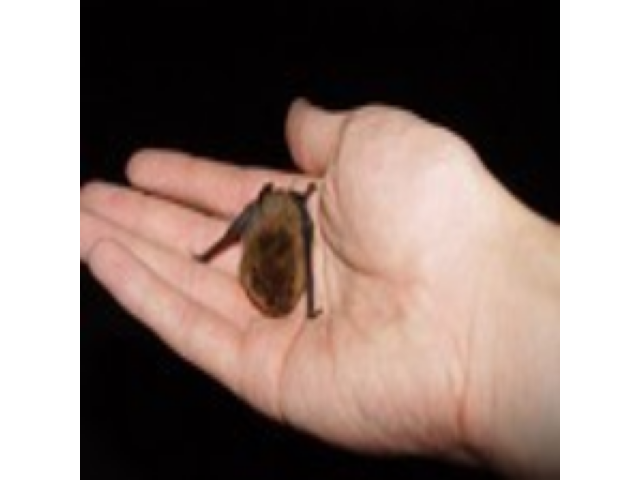
\includegraphics[width=\linewidth]{gt_bug.png}
  \caption{Image of a bug from ImageNet \\segmentation dataset \cite{imagenet-seg}.}\label{fig:gt_bug}
\endminipage\hfill
\minipage{0.5\textwidth}
  \includegraphics[width=\linewidth]{heat_map_bug.png}
  \caption{Segmentation map generated by our ViT- \\base for the bug image.}\label{fig:map_bug}
\endminipage\hfill
\end{figure}

\begin{figure}[H]
\minipage{0.5\textwidth}
  \includegraphics[width=\linewidth]{gt_cow.png}
  \caption{Image of a cow from ImageNet \\segmentation dataset \cite{imagenet-seg}.}\label{fig:gt_cow}
\endminipage\hfill
\minipage{0.5\textwidth}
  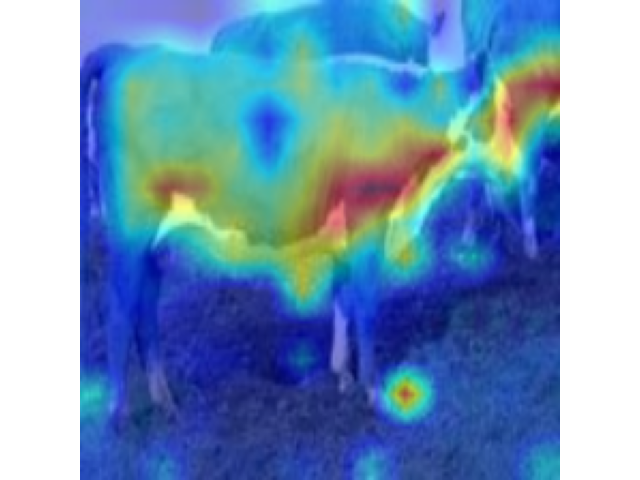
\includegraphics[width=\linewidth]{heat_map_cow.png}
  \caption{Segmentation map generated by our ViT- \\base for the cow image.}\label{fig:map_cow}
\endminipage\hfill
\end{figure}

% \begin{figure}[!h]
% \minipage{0.5\textwidth}
%   \includegraphics[width=\linewidth]{gt_dog.png}
%   \caption{Ground truth segmentation map for \\a dog image from ImageNet \cite{imagenet-seg}.}\label{fig:gt_dog}
% \endminipage\hfill
% \minipage{0.5\textwidth}
%   \includegraphics[width=\linewidth]{heat_map_dog.png}
%   \caption{Segmentation map generated by our ViT- \\base for the dog image.}\label{fig:map_dog}
% \endminipage\hfill
% \end{figure}

\begin{figure}[H]
\minipage{0.5\textwidth}
  \includegraphics[width=\linewidth]{gt_reinder.png}
  \caption{Image of a reindeer from ImageNet \\segmentation dataset \cite{imagenet-seg}.}\label{fig:gt_reinder}
\endminipage\hfill
\minipage{0.5\textwidth}
  \includegraphics[width=\linewidth]{heat_map_reinder.png}
  \caption{Segmentation map generated by our \\ViT-base for the reindeer image.}\label{fig:map_reinder}
\endminipage\hfill
\end{figure}

\begin{figure}[H]
\minipage{0.5\textwidth}
  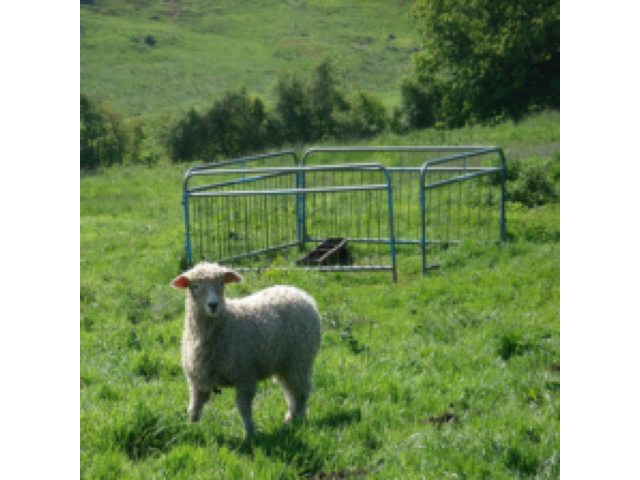
\includegraphics[width=\linewidth]{gt_sheep.png}
  \caption{Image of a sheep from ImageNet \\segmentation dataset \cite{imagenet-seg}.}\label{fig:gt_sheep}
\endminipage\hfill
\minipage{0.5\textwidth}
  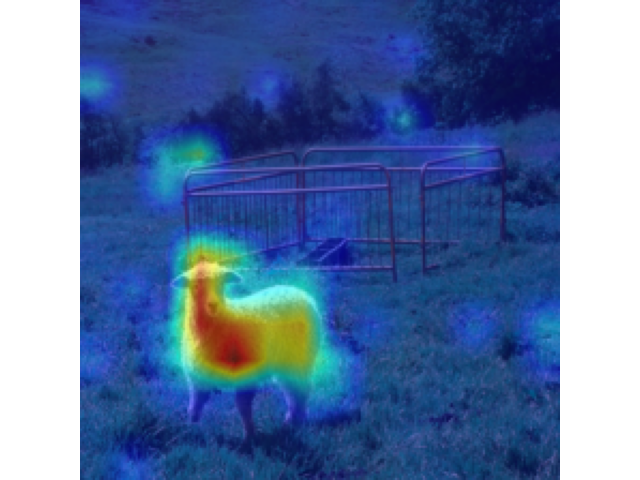
\includegraphics[width=\linewidth]{heat_map_sheep.png}
  \caption{Segmentation map generated by our \\ViT-base for the sheep image.}\label{fig:map_sheep}
\endminipage\hfill
\end{figure}

\begin{figure}[H]
\minipage{0.5\textwidth}
  \includegraphics[width=\linewidth]{gt_squirel.png}
  \caption{Image of a squirrel from ImageNet \\segmentation dataset \cite{imagenet-seg}.}\label{fig:gt_squirel}
\endminipage\hfill
\minipage{0.5\textwidth}
  \includegraphics[width=\linewidth]{heat_map_squirel.png}
  \caption{Segmentation map generated by our \\ViT-base for the squirrel image.}\label{fig:map_squirel}
\endminipage\hfill
\end{figure}

\subsection*{Qualitative Results on Pascal VOC - AffinityNet on Hybrid ViT}
\label{Pascal_results}
In here, we provide qualitative results of the reproduced ViT explainability approach as proposed in \cite{mainpaper}


\begin{figure}[H]
\minipage{0.32\textwidth}
  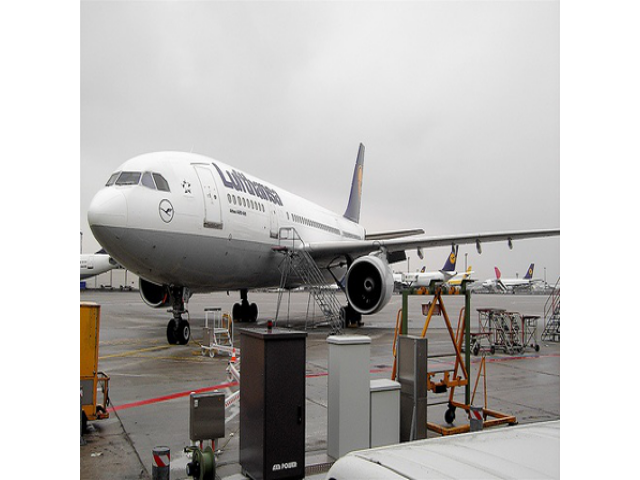
\includegraphics[width=\linewidth]{airplane_gt_affinity.png}
  \caption{Image of an airplane from Pascal VOC segmentation \\dataset \cite{ahn2018learning}.}
  \label{fig:plane_gt}
\endminipage\hfill
\minipage{0.32\textwidth}
  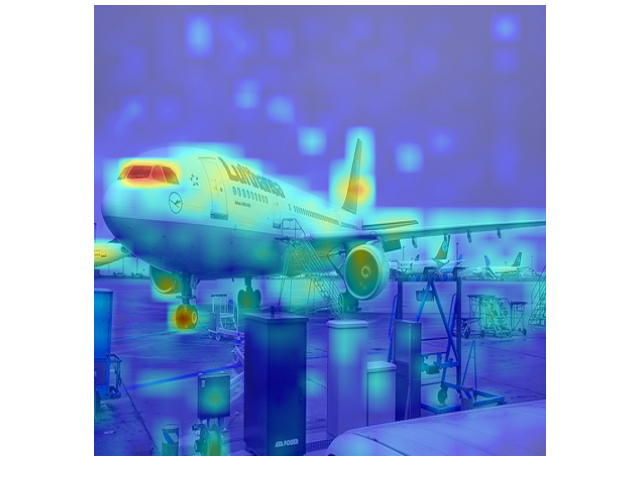
\includegraphics[width=\linewidth]{airplane_heat_map.png}
  \caption{Segmentation map generated by our ViT-base for the airplane image.}
  \label{fig:phane_map}
\endminipage\hfill
\minipage{0.32\textwidth}%
  \includegraphics[width=\linewidth]{plane_affinity.png}
  \caption{Affinity map generated by our AffinityNet for the airplane image.}
  \label{fig:plane_aff}
\endminipage
\end{figure}

\begin{figure}[H]
\minipage{0.32\textwidth}
  \includegraphics[width=\linewidth]{screen_gt.png}
  \caption{Image of an screen from Pascal VOC segmentation \\dataset \cite{ahn2018learning}.}
  \label{fig:screen_gt}
\endminipage\hfill
\minipage{0.32\textwidth}
  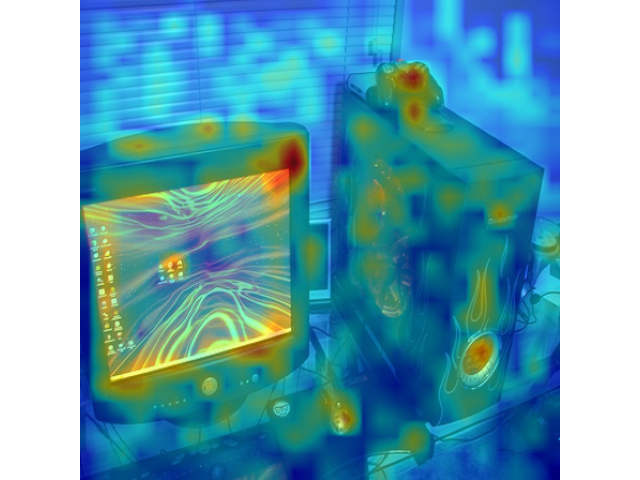
\includegraphics[width=\linewidth]{screen_heat_map.png}
  \caption{Segmentation map generated by our ViT-base for the screen image.}
  \label{fig:screen_map}
\endminipage\hfill
\minipage{0.32\textwidth}%
  \includegraphics[width=\linewidth]{screen_affinity.png}
  \caption{Affinity map generated by our AffinityNet for the screen image.}
  \label{fig:screen_aff}
\endminipage
\end{figure}

\begin{figure}[H]
\minipage{0.32\textwidth}
  \includegraphics[width=\linewidth]{sheep_gt.png}
  \caption{Image of a sheep from Pascal VOC segmentation \\dataset \cite{ahn2018learning}.}
  \label{fig:sheep_gt}
\endminipage\hfill
\minipage{0.32\textwidth}
  \includegraphics[width=\linewidth]{sheep_heat_map.png}
  \caption{Segmentation map generated by our ViT-base for the sheep image.}
  \label{fig:sheep_heat_map}
\endminipage\hfill
\minipage{0.32\textwidth}%
  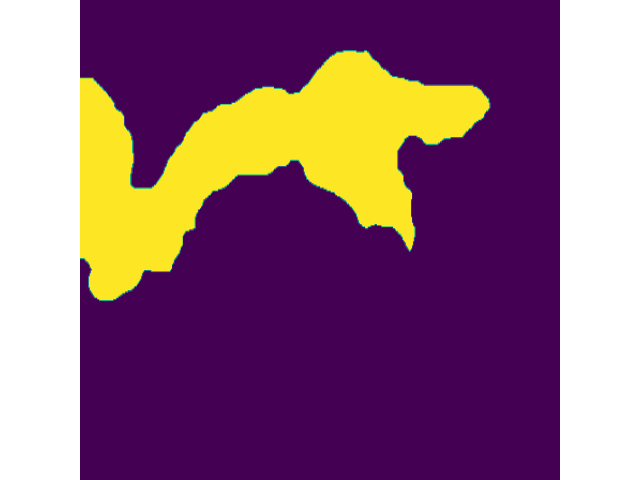
\includegraphics[width=\linewidth]{sheep_affinity.png}
  \caption{Affinity map generated by our AffinityNet for the sheep image.}
  \label{fig:sheep_aff}
\endminipage
\end{figure}

\begin{figure}[H]
\minipage{0.32\textwidth}
  \includegraphics[width=\linewidth]{train_gt.png}
  \caption{Image of a train from Pascal VOC segmentation \\dataset \cite{ahn2018learning}.}
  \label{fig:train_gt}
\endminipage\hfill
\minipage{0.32\textwidth}
  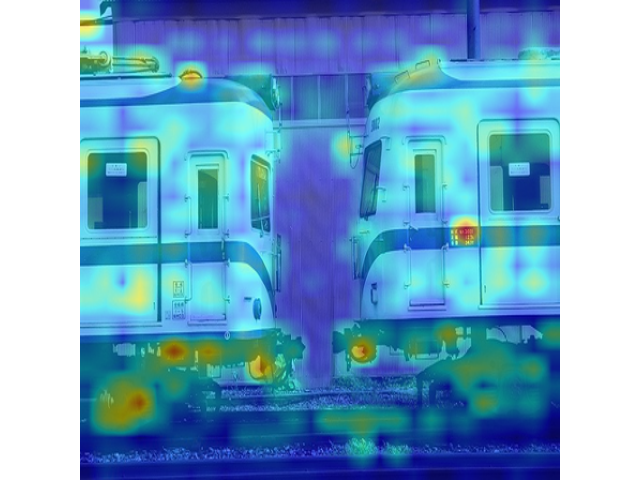
\includegraphics[width=\linewidth]{train_heat_map.png}
  \caption{Segmentation map generated by our ViT-base for the train image.}
  \label{fig:train_heat_map}
\endminipage\hfill
\minipage{0.32\textwidth}%
  \includegraphics[width=\linewidth]{train_affinity.png}
  \caption{Affinity map generated by our AffinityNet for the train image.}
  \label{fig:train_aff}
\endminipage
\end{figure}

\newpage

\bibliographystyle{ieeetr}
\bibliography{reflist}

\end{document}